\documentclass{beamer}

\usetheme[white,sections]{Wisconsin}
\usepackage{fancyvrb}
\usepackage{color}
\usepackage[normalem]{ulem}
\usepackage{xcolor}
\usepackage{anyfontsize}
\usepackage[belowskip=-15pt,aboveskip=0pt]{caption}
\usepackage{amsmath}
\usepackage{color}
\usepackage{listings}
\lstset{ %
language=matlab,                % choose the language of the code
basicstyle=\footnotesize,       % the size of the fonts that are used for the code
numbers=left,                   % where to put the line-numbers
numberstyle=\footnotesize,      % the size of the fonts that are used for the line-numbers
stepnumber=1,                   % the step between two line-numbers. If it is 1 each line will be numbered
numbersep=5pt,                  % how far the line-numbers are from the code
backgroundcolor=\color{white},  % choose the background color. You must add \usepackage{color}
showspaces=false,               % show spaces adding particular underscores
showstringspaces=false,         % underline spaces within strings
showtabs=false,                 % show tabs within strings adding particular underscores
frame=single,           % adds a frame around the code
tabsize=2,          % sets default tabsize to 2 spaces
captionpos=b,           % sets the caption-position to bottom
breaklines=true,        % sets automatic line breaking
breakatwhitespace=false,    % sets if automatic breaks should only happen at whitespace
escapeinside={\%*}{*},          % if you want to add a comment within your code
moredelim=**[is][\color{red}]{@}{@}
}

\begin{document}
\newcommand*{\alphabet}{ABCDEFGHIJKLMNOPQRSTUVWXYZabcdefghijklmnopqrstuvwxyz}
\newlength{\highlightheight}
\newlength{\highlightdepth}
\newlength{\highlightmargin}
\setlength{\highlightmargin}{2pt}
\settoheight{\highlightheight}{\alphabet}
\settodepth{\highlightdepth}{\alphabet}
\addtolength{\highlightheight}{\highlightmargin}
\addtolength{\highlightdepth}{\highlightmargin}
\addtolength{\highlightheight}{\highlightdepth}
\setbeamertemplate{bibliography entry title}{}
\setbeamertemplate{bibliography entry location}{}
\setbeamertemplate{bibliography entry note}{}
\newcommand*{\Highlight}{\rlap{\textcolor{HighlightBackground}{\rule[-\highlightdepth]{\linewidth}{\highlightheight}}}}
\setbeamertemplate{bibliography item}[text]
\setbeamercolor{section in toc}{fg=white}
\setbeamercolor{bibliography entry author}{fg=black}
\setbeamercolor{bibliography item}{fg=black}
\setbeamercolor*{bibliography entry title}{fg=black}
%\setbeamerfont{section number projected}{size=\tiny}
\setbeamerfont{section number projected}{size=\fontsize{6}{6}\selectfont}
%\setbeamerfont{toc}{color=white}
\setbeamerfont{itemize/enumerate subbody}{size=\Large}
\setbeamercolor{section number projected}{bg=UWRed,fg=white}
\setbeamercolor{subsection number projected}{bg=UWRed,fg=white}
\hypersetup{linkcolor=white,urlcolor=white}

%%%%%%%%%%%%%%%%%%%%%%%%%%%%%%%%%%%%%%%%%%%%%%%%%%%%%%%%%%%%%%%%%%%%%%%%%%
%%%%%%%%%%%%%%%%%%%%%%%%%%%%%%%%%%%%%%%%%%%%%%%%%%%%%%%%%%%%%%%%%%%%%%%%%%
%%%%%%%%%%%%%%%%%%%%%%%%%%%%%%%%%%%%%%%%%%%%%%%%%%%%%%%%%%%%%%%%%%%%%%%%%%
% START DOCUMENT
%%%%%%%%%%%%%%%%%%%%%%%%%%%%%%%%%%%%%%%%%%%%%%%%%%%%%%%%%%%%%%%%%%%%%%%%%%
%%%%%%%%%%%%%%%%%%%%%%%%%%%%%%%%%%%%%%%%%%%%%%%%%%%%%%%%%%%%%%%%%%%%%%%%%%
%%%%%%%%%%%%%%%%%%%%%%%%%%%%%%%%%%%%%%%%%%%%%%%%%%%%%%%%%%%%%%%%%%%%%%%%%%
%%%%%%%%%%%%%%%%%%%%%%%%%%%%%%%%%%%%%%%%%%%%%%%%%%%%%%%%%%%%%%%%%%%%%%%%%%

%TITLE PAGE
%%%%%%%%%%%%%%%%%%%%%%%%%%%%%%%%%%%%%%%%%%%%%%%%%%%%%%%%%%%%%%%%%%%%%%%%%%%%%%%%
\title{ME759 Final Presentation: Diagonally Dominant Banded Systems Solving in Parallel}
\author{Elliott Biondo}
\institute{University of Wisconsin - Madison}
\date{December 19, 2013}
\frame[plain]{\titlepage \addtocounter{framenumber}{-1}}
\Large
%%%%%%%%%%%%%%%%%%%%%%%%%%%%%%%%%%%%%%%%%%%%%%%%%%%%%%%%%%%%%%%%%%%%%%%%%%%%%%%%
\begin{frame}
\frametitle{Summary of work}

\begin{itemize}
\item{Solving banded, diagonally dominant, linear systems.}
\item{CUDA implementation.}
\item{OpenMP implementation.}
\item{Comparison to Intel MKL \texttt{LAPACKE\_dgbsv}}
\end{itemize}

\end{frame}
%%%%%%%%%%%%%%%%%%%%%%%%%%%%%%%%%%%%%%%%%%%%%%%%%%%%%%%%%%%%%%%%%%%%%%%%%%%%%%%%

\begin{frame}[fragile]
\frametitle{Overview}
\setbeamercolor{section in toc}{fg=black}
\setbeamercolor{subsection in toc}{fg=black}
\setbeamerfont{section number projected}{size=\fontsize{11}{11}\selectfont}
\setbeamercolor{subsection number projected}{bg=UWRed,fg=white}

\setbeamerfont{subsection number projected}{size=\fontsize{11}{11}\selectfont}
 \tableofcontents[sectionstyle=show,subsectionstyle=show]
\end{frame}

%%%%%%%%%%%%%%%%%%%%%%%%%%%%%%%%%%%%%%%%%%%%%%%%%%%%%%%%%%%%%%%%%%%%%%%%
%%%%%%%%%%%%%%%%%%%%%%%%%%%%%%%%%%%%%%%%%%%%%%%%%%%%%%%%%%%%%%%%%%%%%%%%
%%%%%%%%%%%%%%%%%%%%%%%%%%%%%%%%%%%%%%%%%%%%%%%%%%%%%%%%%%%%%%%%%%%%%%%%
\section{Algorithm}
%%%%%%%%%%%%%%%%%%%%%%%%%%%%%%%%%%%%%%%%%%%%%%%%%%%%%%%%%%%%%%%%%%%%%%%%
\begin{frame}
\frametitle{Algorithm}
$$
Ax=b
$$
Matrix assumed to be symmetric, with bandwidth:
$$
k = 2 \cdot k_{1/2} + 1
$$

LU Decomposition
$$
A = LU
$$

Forward substitution:
$$
Ly_i = b_i
$$

Backward substitution:
$$
Ux_i = y_i
$$
\end{frame}
%%%%%%%%%%%%%%%%%%%%%%%%%%%%%%%%%%%%%%%%%%%%%%%%%%%%%%%%%%%%%%%%%%%%%%%%
 \begin{frame}[fragile]{LU decomposition}

\begin{lstlisting}
  for i = 0 .. n-2
    for j = i+1 .. n-1
      A[j][i] = A[j][i]/A[i][i]
    end
    for j = i+1 .. n-1
      for k = i+1 .. n-1
        A[j][k] = A[j][k] - A[j][i]*A[i][k]
      end
    end
  end
\end{lstlisting}

\centerline{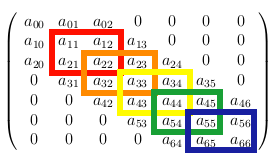
\includegraphics[width=5cm]{active_region_colored2.png}}

\end{frame}
%%%%%%%%%%%%%%%%%%%%%%%%%%%%%%%%%%%%%%%%%%%%%%%%%%%%%%%%%%%%%%%%%%%%%%%
 \begin{frame}[fragile]{Forward/backward substitution}
\begin{lstlisting}
  for i = 0 .. n-1
    for j = i+1 .. n-1
      b[j] = b[j] - b[i]*A[j][i]
    end
  end
\end{lstlisting}

\begin{lstlisting}
  for i = n-1 .. 0
    b[i] = b[i]/A[i][i]
    for j = 0 .. i-1
      b[j] = b[j] - b[i]*A[j][i]
    end
  end
\end{lstlisting}

\end{frame}
%%%%%%%%%%%%%%%%%%%%%%%%%%%%%%%%%%%%%%%%%%%%%%%%%%%%%%%%%%%%%%%%%%%%%%%%
\begin{frame}
\frametitle{Band storage}
\centering

\begin{itemize}
\item{Reduce storage requirement from $N \cdot N$ to $N \cdot k$.}
\end{itemize}

\vspace{1cm}
{\normalsize
$$
\left(
\begin{array}{c c c c c c c}
a_{00} & a_{01} & a_{02} & 0 & 0 & 0 & 0\\
a_{10} & a_{11} & a_{12} & a_{13} & 0 & 0 & 0\\
a_{20} & a_{21} & a_{22} & a_{23} & a_{24} & 0 & 0\\
     0 & a_{31} & a_{32} & a_{33} & a_{34} & a_{35} & 0\\
     0 &      0 & a_{42} & a_{43} & a_{44} & a_{45} & a_{46}\\
     0 &      0 &      0 & a_{53} & a_{54} & a_{55} & a_{56}\\
     0 &      0 &      0 &      0 & a_{64} & a_{65} & a_{66}\\
\end{array}
\right)
\rightarrow
\left(
\begin{array}{c c c c c}
     0 &      0 & a_{00} & a_{01} & a_{02}\\
     0 & a_{10} & a_{11} & a_{12} & a_{13}\\
a_{20} & a_{21} & a_{22} & a_{23} & a_{24}\\
a_{31} & a_{32} & a_{33} & a_{34} & a_{35}\\
a_{42} & a_{43} & a_{44} & a_{45} & a_{46}\\
a_{53} & a_{54} & a_{55} & a_{56} & 0     \\
a_{64} & a_{65} & a_{66} & 0      & 0
\end{array}
\right)
$$
}



\end{frame}
%%%%%%%%%%%%%%%%%%%%%%%%%%%%%%%%%%%%%%%%%%%%%%%%%%%%%%%%%%%%%%%%%%%%%%%%
%%%%%%%%%%%%%%%%%%%%%%%%%%%%%%%%%%%%%%%%%%%%%%%%%%%%%%%%%%%%%%%%%%%%%%%%
%%%%%%%%%%%%%%%%%%%%%%%%%%%%%%%%%%%%%%%%%%%%%%%%%%%%%%%%%%%%%%%%%%%%%%%%
\section{CUDA}
%%%%%%%%%%%%%%%%%%%%%%%%%%%%%%%%%%%%%%%%%%%%%%%%%%%%%%%%%%%%%%%%%%%%%%%%
\begin{frame}
\frametitle{CUDA}
\begin{itemize}
\item{Features:
  \begin{itemize}
  \item{Only stores and operates on band.}
  \item{Parallelization of all 3 major steps.}
  \item{Utilization of shared memory.}
  \item{Pinned host memory.}
  \item{Support of multiple RHS.}
  \item{Production mode for solving user-supplied systems.}
  \end{itemize}
}
\end{itemize}
  \end{frame}
%%%%%%%%%%%%%%%%%%%%%%%%%%%%%%%%%%%%%%%%%%%%%%%%%%%%%%%%%%%%%%%%%%%%%%%%
\begin{frame}
\frametitle{Comparison to Intel MKL}
Execution times for different \% bandwidths.
\centerline{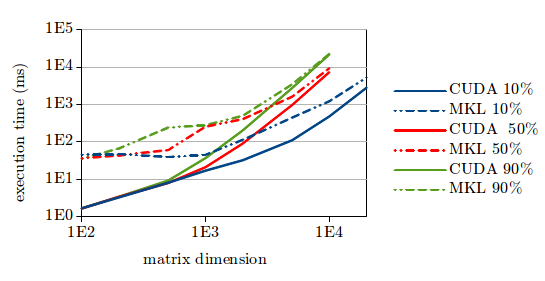
\includegraphics[width=8cm]{full_scaling.png}}
\end{frame}

\begin{frame}
\frametitle{RHS Scaling}
{\small
Matrix dimension kept constant at 1000 with a bandwidth of 501.}
\vspace*{-0.1cm}
\begin{figure}[H]
\label{rhs}
\centerline{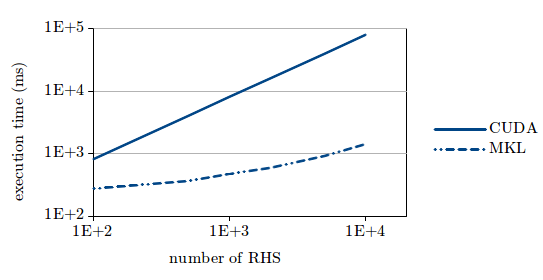
\includegraphics[width=7cm]{rhs.png}}
\end{figure}
\vspace{-1.1cm}

{\small NVVP with matrix dimension of 1000 bandwidth of 501 and 10 RHS.}
\vspace{0.1cm}
\centerline{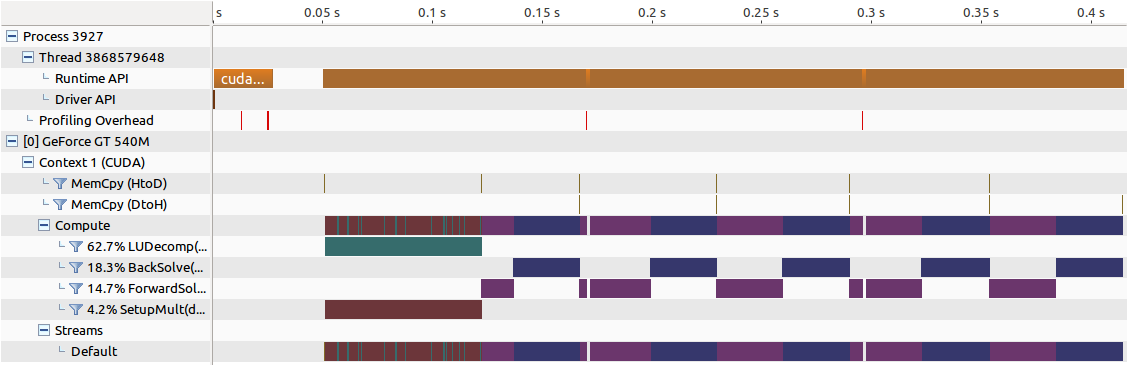
\includegraphics[width=9cm]{nvvp.png}}

\end{frame}

%%%%%%%%%%%%%%%%%%%%%%%%%%%%%%%%%%%%%%%%%%%%%%%%%%%%%%%%%%%%%%%%%%%%%%%%
%%%%%%%%%%%%%%%%%%%%%%%%%%%%%%%%%%%%%%%%%%%%%%%%%%%%%%%%%%%%%%%%%%%%%%%%
%%%%%%%%%%%%%%%%%%%%%%%%%%%%%%%%%%%%%%%%%%%%%%%%%%%%%%%%%%%%%%%%%%%%%%%%
\section{OpenMP}
%%%%%%%%%%%%%%%%%%%%%%%%%%%%%%%%%%%%%%%%%%%%%%%%%%%%%%%%%%%%%%%%%%%%%%%%
\begin{frame}
\frametitle{OpenMP features}
\begin{itemize}
\item{Only stores and operates on band.}
\item{Parallelization of solving multiple RHS.}
\item{Based on serial implementation.}
\end{itemize}
\end{frame}
%%%%%%%%%%%%%%%%%%%%%%%%%%%%%%%%%%%%%%%%%%%%%%%%%%%%%%%%%%%%%%%%%%%%%%%%
\begin{frame}[fragile]
\frametitle{First attempt}

Parallelize active region:
\begin{lstlisting}
  for i = 0 .. n-2
    for j = i+1 .. n-1
      A[j][i] = A[j][i]/A[i][i]
    end
   @for j = i+1 .. n-1@
     @for k = i+1 .. n-1@
       @A[j][k] = A[j][k] - A[j][i]*A[i][k]@
     @end@
   @end@
  end
\end{lstlisting}

Problem: Thread creating takes place $N-2$ times.
\end{frame}

%%%%%%%%%%%%%%%%%%%%%%%%%%%%%%%%%%%%%%%%%%%%%%%%%%%%%%%%%%%%%%%%%%%%%%%%
\begin{frame}
\frametitle{Scaling}


\centerline{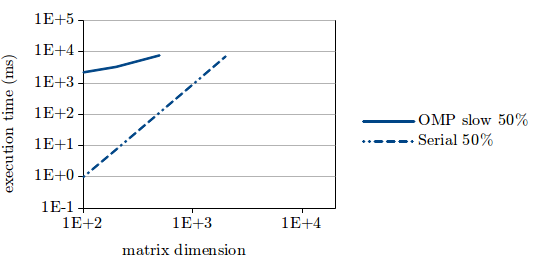
\includegraphics[width=12cm]{slow.png}}

\end{frame}

%%%%%%%%%%%%%%%%%%%%%%%%%%%%%%%%%%%%%%%%%%%%%%%%%%%%%%%%%%%%%%%%%%%%%%%%
\begin{frame}[fragile]
\frametitle{Second attempt}
Parallelize solving of $w$ RHS.
\begin{lstlisting}
for u = 0 .. w - 1
    # forward substitution
    for i = 0 .. n-1
      for j = i+1 .. n-1
        b[j] = b[j] - b[i]*A[j][i]
      end
    end
   # backward substitution
    for i = n-1 .. 0
      b[i] = b[i]/A[i][i]
      for j = 0 .. i-1
        b[j] = b[j] - b[i]*A[j][i]
      end
    end
end
\end{lstlisting}
\end{frame}
%%%%%%%%%%%%%%%%%%%%%%%%%%%%%%%%%%%%%%%%%%%%%%%%%%%%%%%%%%%%%%%%%%%%%%%%
\begin{frame}
\frametitle{RHS scaling}
\centerline{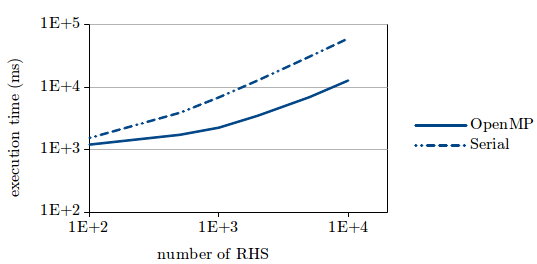
\includegraphics[width=12cm]{omp_rhs.png}}
\end{frame}
%%%%%%%%%%%%%%%%%%%%%%%%%%%%%%%%%%%%%%%%%%%%%%%%%%%%%%%%%%%%%%%%%%%%%%%%
%%%%%%%%%%%%%%%%%%%%%%%%%%%%%%%%%%%%%%%%%%%%%%%%%%%%%%%%%%%%%%%%%%%%%%%%
%%%%%%%%%%%%%%%%%%%%%%%%%%%%%%%%%%%%%%%%%%%%%%%%%%%%%%%%%%%%%%%%%%%%%%%%
\section{Conclusions}
\begin{frame}
\frametitle{Conclusions}
\begin{itemize}
\item{CUDA is extremely versatile and well-suited for fine grain parallelism.
     \begin{itemize}
     \item{Added layer of complexity with thread indexing.}
     \end{itemize}
     }
\item{OpenMP threads are bulkier, and may require different algorithms than CUDA.
     \begin{itemize}
     \item{Trivial to implement.}
     \end{itemize}
     }
\item{Highly optimized serial code rivals parallel code.}
\end{itemize}
\end{frame}
%%%%%%%%%%%%%%%%%%%%%%%%%%%%%%%%%%%%%%%%%%%%%%%%%%%%%%%%%%%%%%%%%%%%%%%%%%%%%%%%
%%%%%%%%%%%%%%%%%%%%%%%%%%%%%%%%%%%%%%%%%%%%%%%%%%%%%%%%%%%%%%%%%%%%%%%%%%%%%%%%
%%%%%%%%%%%%%%%%%%%%%%%%%%%%%%%%%%%%%%%%%%%%%%%%%%%%%%%%%%%%%%%%%%%%%%%%%%%%%%%%
%%%%%%%%%%%%%%%%%%%%%%%%%%%%%%%%%%%%%%%%%%%%%%%%%%%%%%%%%%%%%%%%%%%%%%%%%%%%%%%%
\end{document}
%%%%%%%%%%%%%%%%%%%%%%%%%%%%%%%%%%%%%%%%%%%%%%%%%%%%%%%%%%%%%%%%%%%%%%%%%%%%%%%%
%%%%%%%%%%%%%%%%%%%%%%%%%%%%%%%%%%%%%%%%%%%%%%%%%%%%%%%%%%%%%%%%%%%%%%%%%%%%%%%%
